\documentclass[10pt,a4paper]{article}
\usepackage[utf8]{inputenc}
\usepackage{amsmath}
\usepackage{amsfonts}
\usepackage{amssymb}
\usepackage{amsthm}

\usepackage{float}
\usepackage{subfigure}
\usepackage{framed}
\usepackage{xcolor}

\usepackage{hyperref}
\hypersetup{
  colorlinks   = true, %Colours links instead of ugly boxes
  urlcolor     = red, %Colour for external hyperlinks
  linkcolor    = blue, %Colour of internal links
  citecolor   = blue %Colour of citations
}

\usepackage{graphicx}
\graphicspath{{images2/}}

\definecolor{shadecolor}{gray}{0.9}

\newtheorem{questions}{Question}
\newenvironment{question}
   {\begin{shaded}\begin{questions}}
   {\end{questions}\end{shaded}}

\author{Ram\'on Mart\'inez}
\title{BCPNN and Sequence Learning}

% Paragraph parameters
\setlength{\parskip}{1em}

\begin{document}
\maketitle

\section{Results}
\begin{figure}[H]
\centering
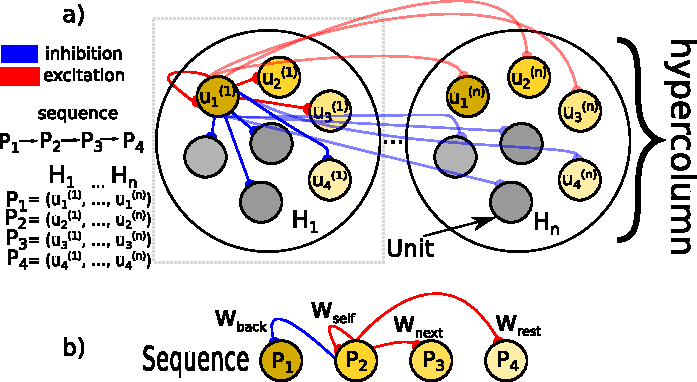
\includegraphics[scale=1.0]{diagram.pdf}
\caption{A diagram }
\label{fig:networks_scheme}
\end{figure}


\begin{align}
\tau_s \dfrac{ds_i}{dt} &= g_{beta}\beta_i + \sum_{j} w_{ij} o_j  - g_a a_i - s_i  + \xi(t) \label{eq:simple_bcpnn} \\ 
o_i &=  \delta_{i, argmax(s)} \label{eq:simple_bcpnn_max} \\ 
\tau_a \dfrac{da_i}{dt} &= o_i - a_i \label{eq:simple_bcpnn_adaptation}
\end{align}


\subsection{The system can recall sequences}
\section{Results}
\begin{figure}[H]
\centering
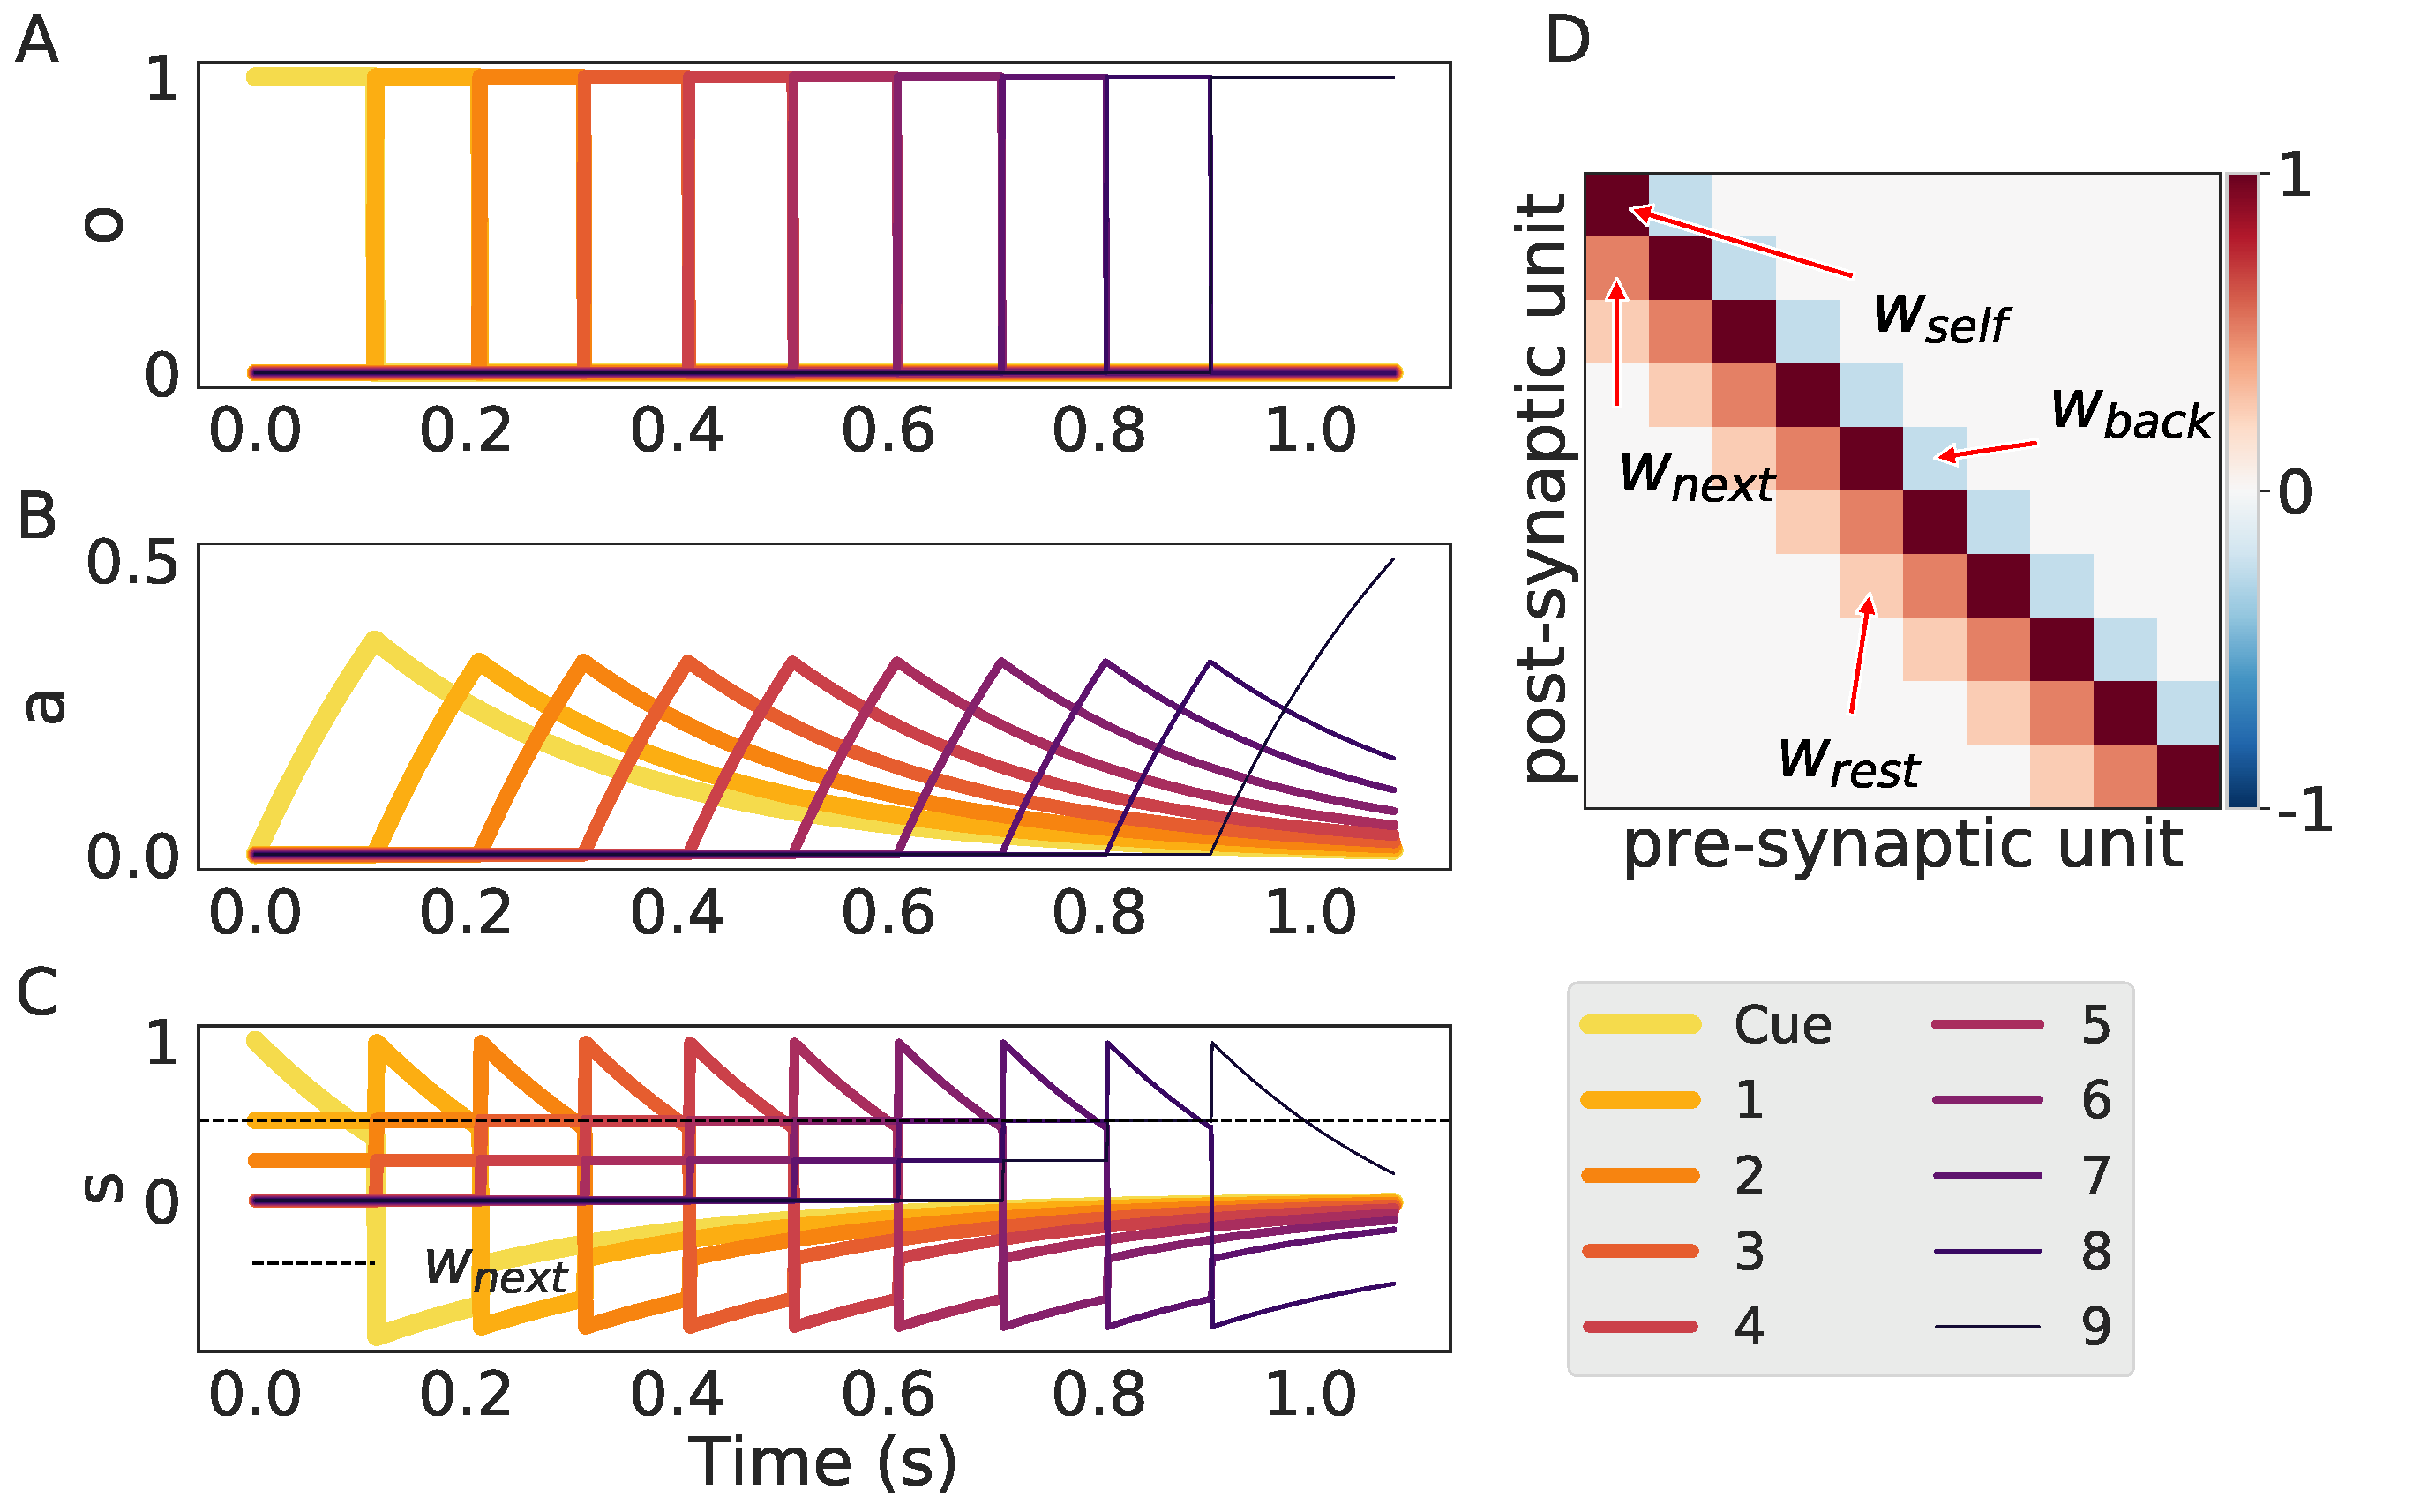
\includegraphics[scale=0.25]{simple_bcpnn_recall.pdf}
\caption{An example of recall}
\label{fig:recall}
\end{figure}

\subsubsection{Analytical solution}
We can solve the deterministic equations analytical with the method of undetermined coefficients. There are two conditions, the unit that is active, and the unit that is not. 


\begin{align*} 
s(t) &= I_{fix} - g_a\left(\frac{C_{charge}}{1 - r} \right) e^{-\frac{t}{\tau_a}} + \left(s_0 - I_{fix} + g_a \left( \frac{C_{charge}}{1 - r}\right)\right)e^{-\frac{t}{\tau_s}} \\
s(t) &= \beta + w - g_a + g_a \left(\frac{1 - a_0}{1 - r}\right) e^{-\frac{t}{\tau_a}} + \left(s_0 - \beta - w + g_a - g_a \frac{1 - a_0}{1 - r}\right) e^{-\frac{t}{\tau_s}}  \\ 
s(t) &= \beta + w - g_a \left( \frac{a_0}{1 - r} \right) e^{-\frac{t}{\tau_a}} + \left(s_0 - \beta  - w  + g_a \left( \frac{a_0}{1 - r} \right) \right) e^{-\frac{t}{\tau_s}} 
\end{align*}

Where $r=\frac{\tau_s}{\tau_a}$ and $C_{charge}=a_0$ for the non-active case and $C_{charge} = a_0 - 1$ for the active case. Same for $I_{fix}=\beta + w$ for the non-active case and $I_{fix} = \beta + w - g_a$ for the active case. 

\subsection{Persistent time}
\begin{figure}[H]
\centering
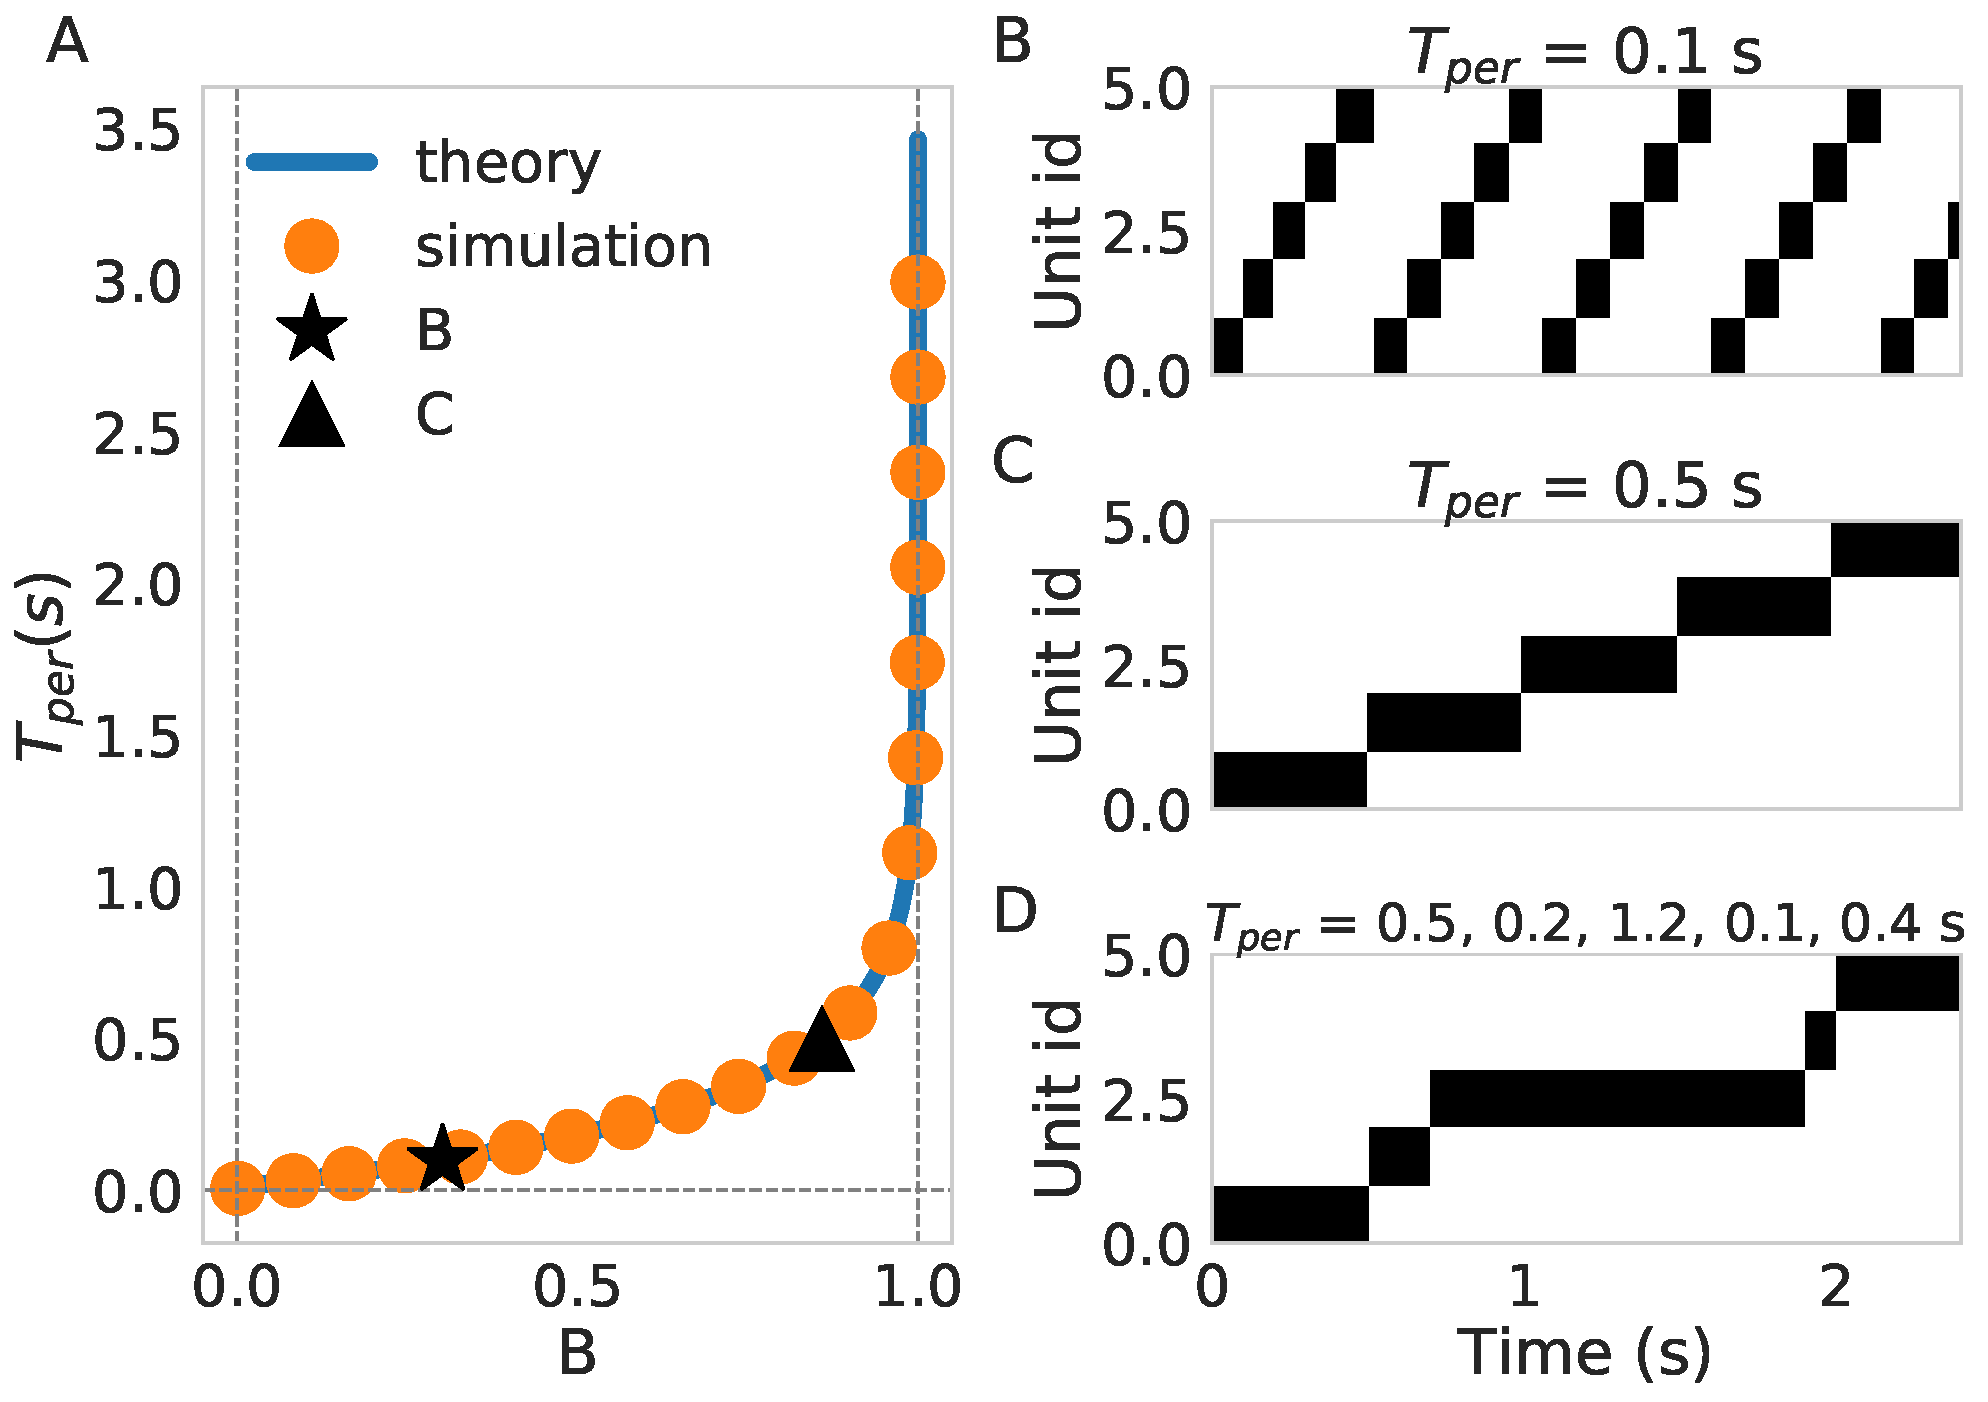
\includegraphics[scale=0.25]{persistent_times.pdf}
\caption{A characterization of persistent times}
\label{fig:per_time}
\end{figure}

We write now for completion the expressions of homogeneous parameters:

\begin{align*}
\frac{T_{ij}}{\tau_a} = \log \left(\frac{1}{1 - B_{ij}} \right) + \log \left( \frac{1}{1 - r} \right) + \log \bigg( a_i(0) + (1 - a_j(0)) \bigg) 
\end{align*}

The second term is of the order of $\tau_s$ usually and the third term accounts for memory effects on the adaptation.

Where $B_{ij} = \frac{w_{jj} - w_{ij} + \beta_j - \beta_i}{g_j}$ is a measure of inertia or inverse of speed. The close to one it is, the longer the transition takes. Also, we see that $B_{ij}$ needs to be bigger than 0 for the transition to occur, from there we can derive the criteria that $g_j > \delta w + \delta \beta$. We also introduced the short hand $f_i = \frac{1}{1 - r_i}$ which is always bigger than 1 for this system and it represents delay effects introduced due to the capacitive nature of the unit.  We see that the presence of adaptive current in the unit that is active hastens the transition ($a_j(0) > 0$  makes $T_{ij}$ smaller by reducing the second term inside the second logarithm). On the other hand, the presence of adaptive current on the next unit ($a_i(0) > 0$) in the sequence slows the process by increasing the first term in the second logarithm. 

\subsection{Learning}
\begin{figure}[H]
\centering
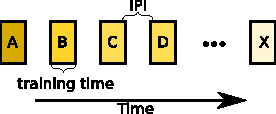
\includegraphics[scale=1.40]{protocol.pdf}
\caption{The training protocol. IPI stands for inter pulse interval and ISI for inter sequence interval. Explanations in the text.}
\label{fig:training_protocol}
\end{figure}


\begin{figure}[H]
\centering
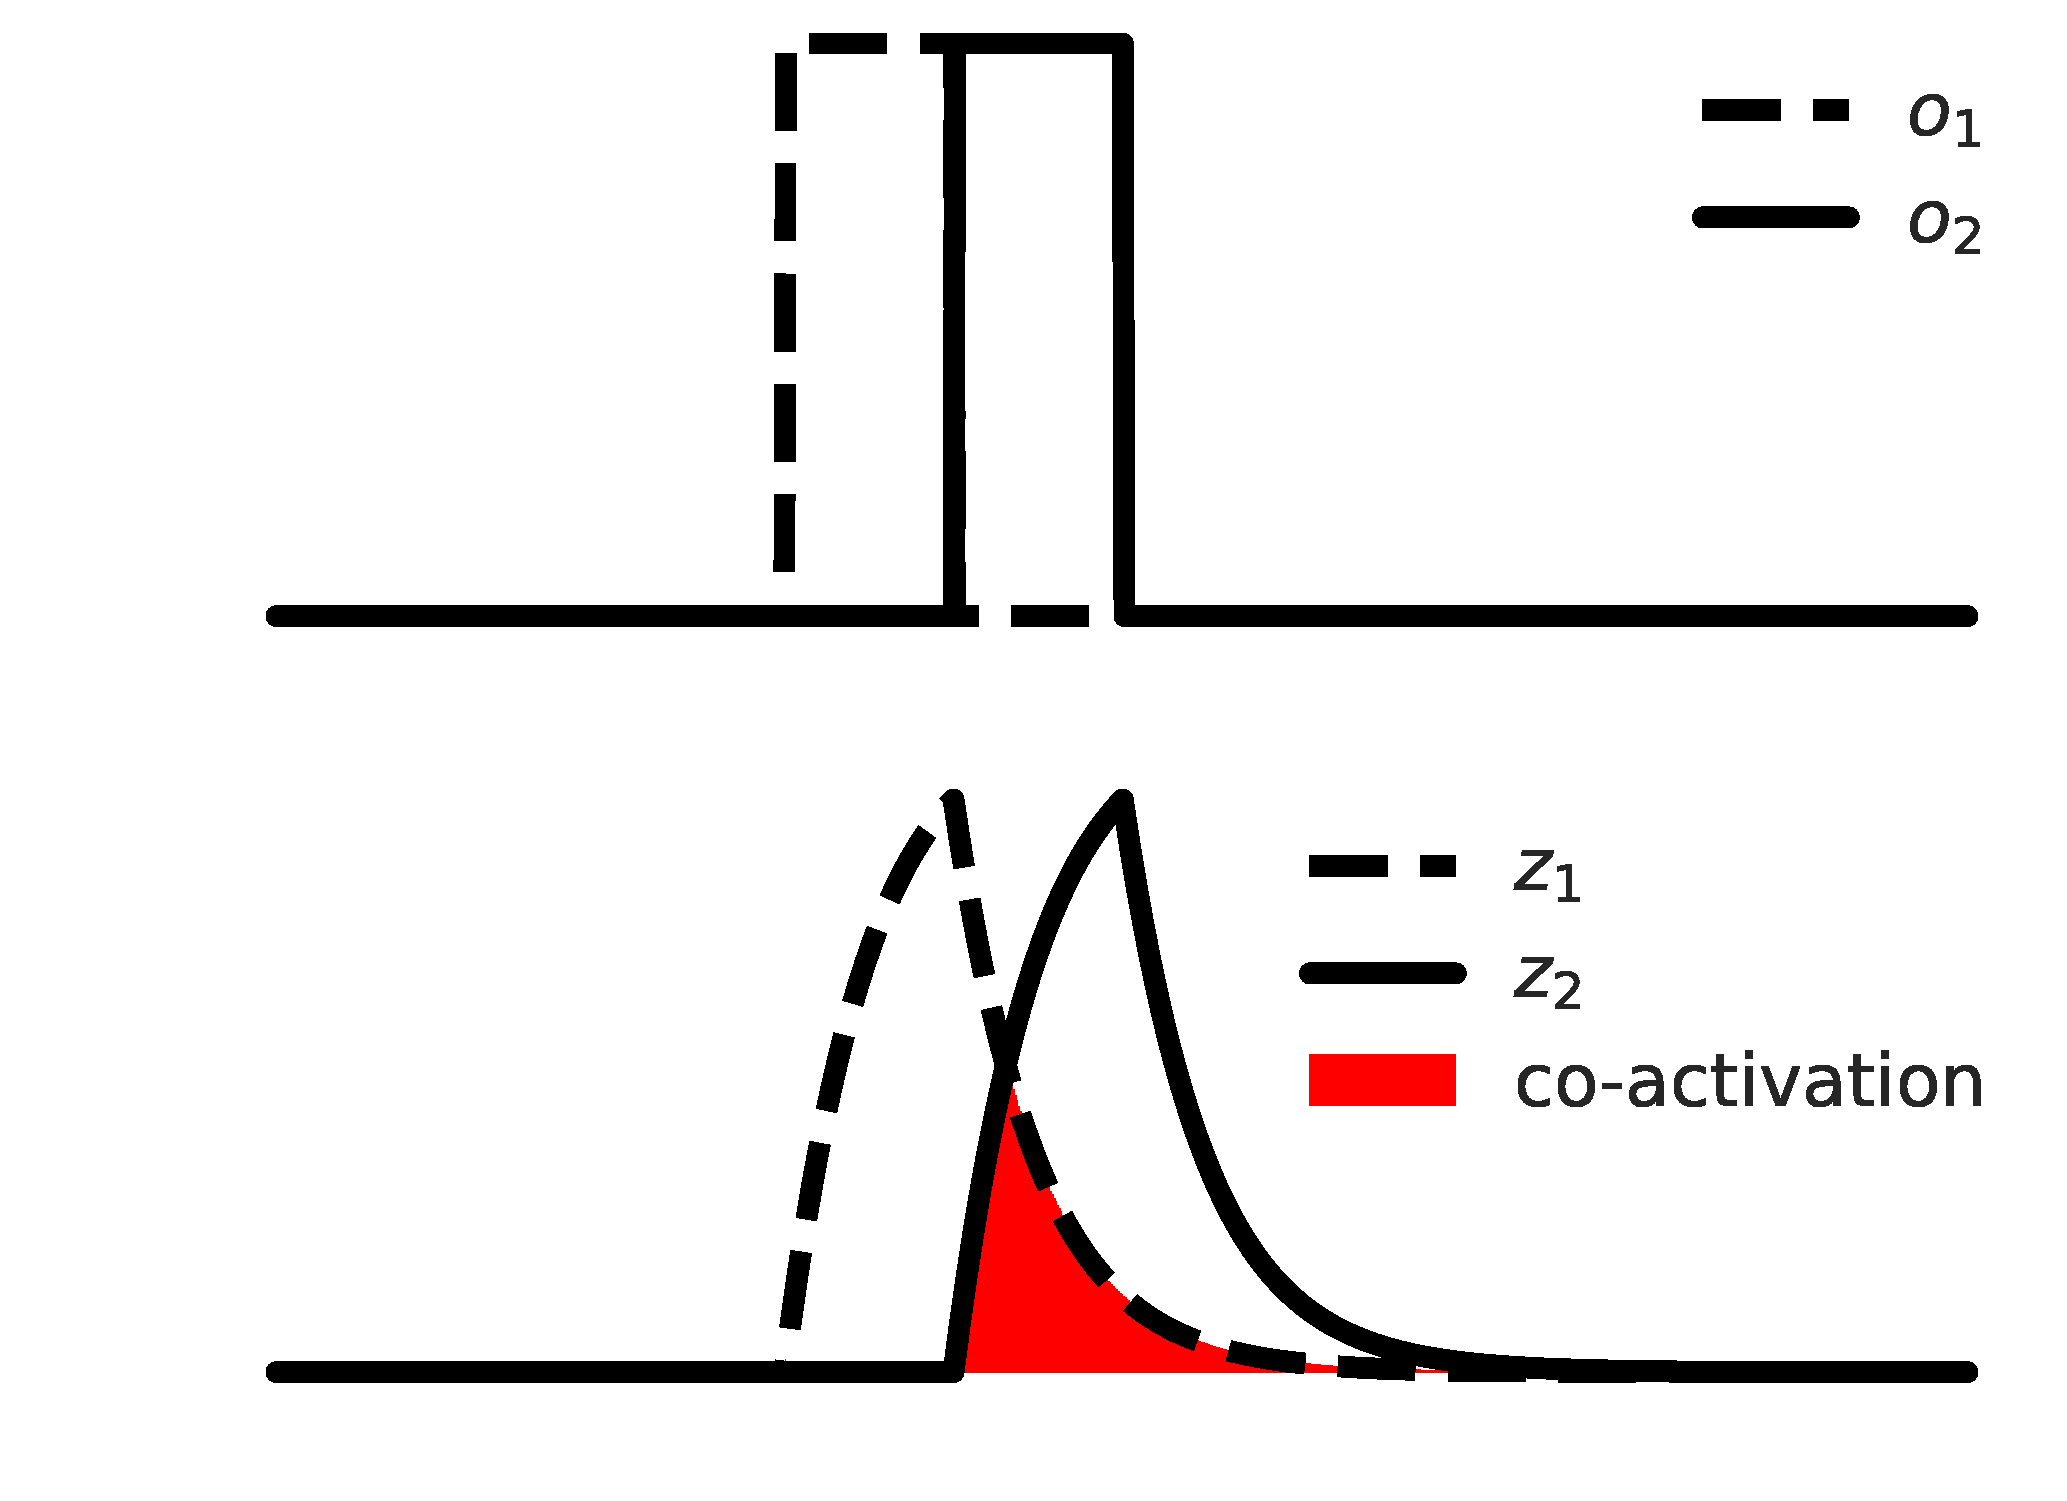
\includegraphics[scale=0.30]{traces_example.pdf}
\caption{In red the intersection of two traces (co-activation) weighted against the base activation rate of each unit is responsible for the increase or decrease on the connectivity weight.}
\label{fig:traces_example}
\end{figure}

\begin{figure}[H]
\centering
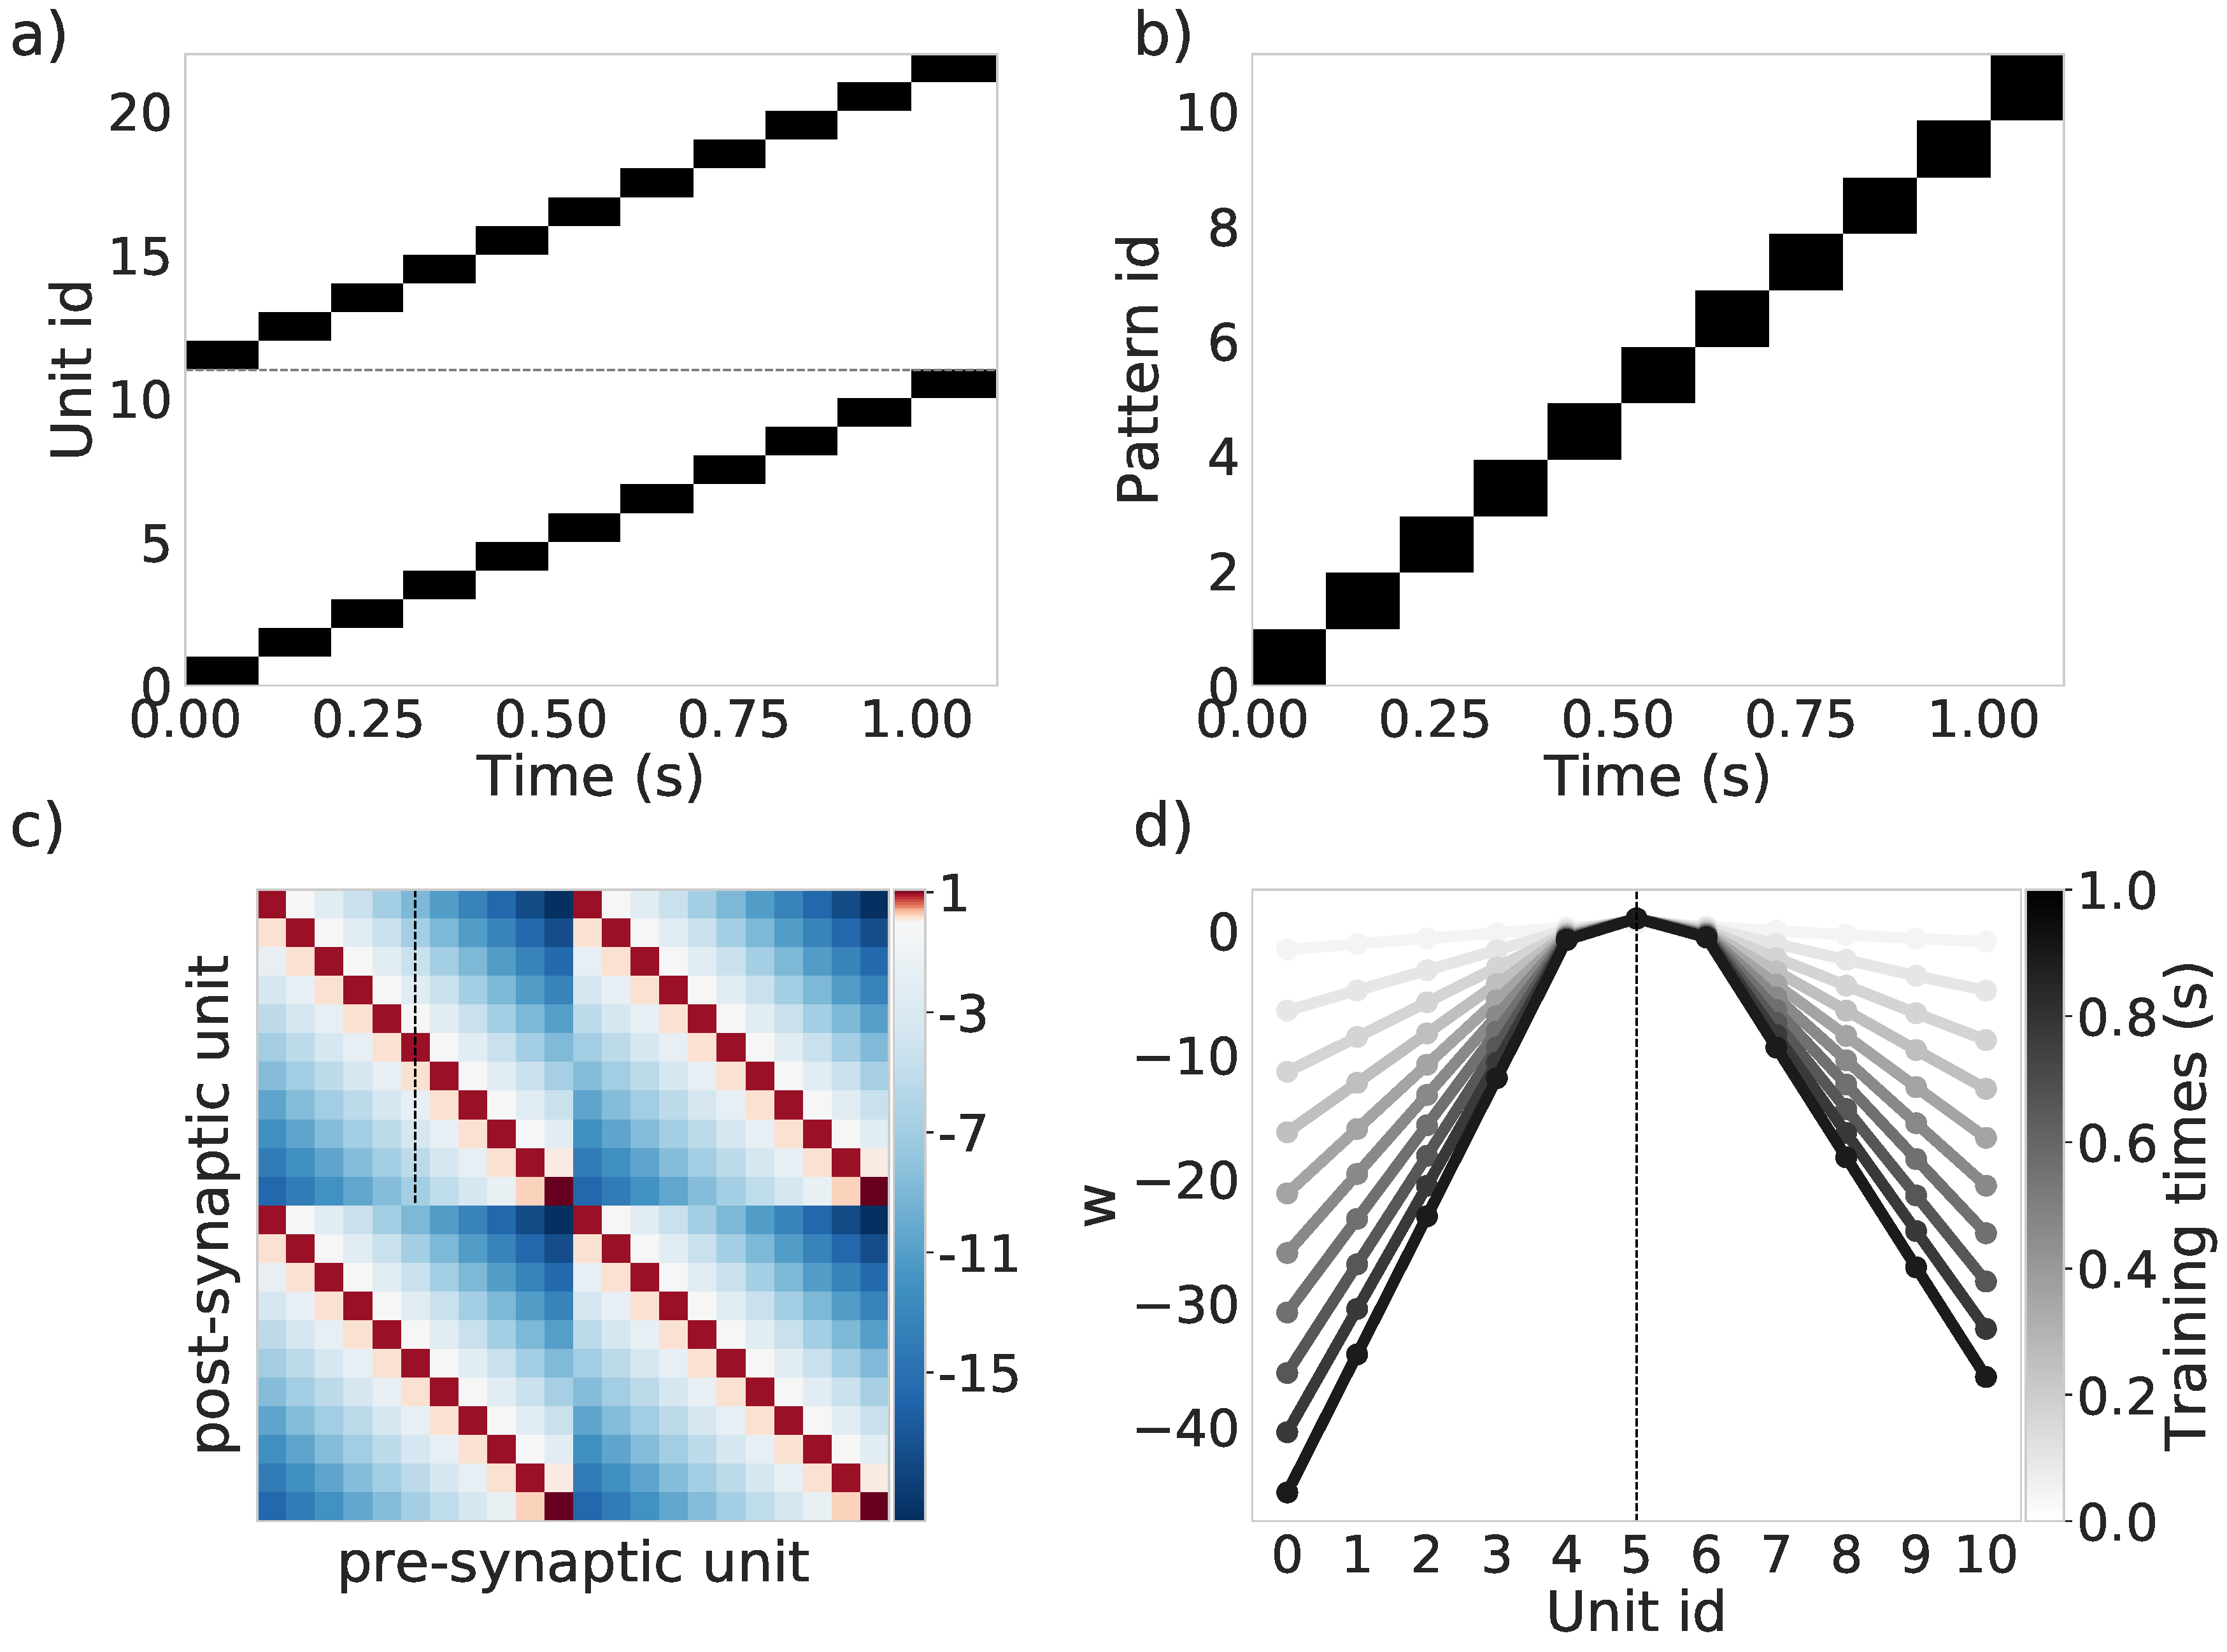
\includegraphics[scale=0.15]{recall_example.pdf}
\caption{A recall example}
\label{fig:recall_example}
\end{figure}

\begin{figure}[H]
\centering
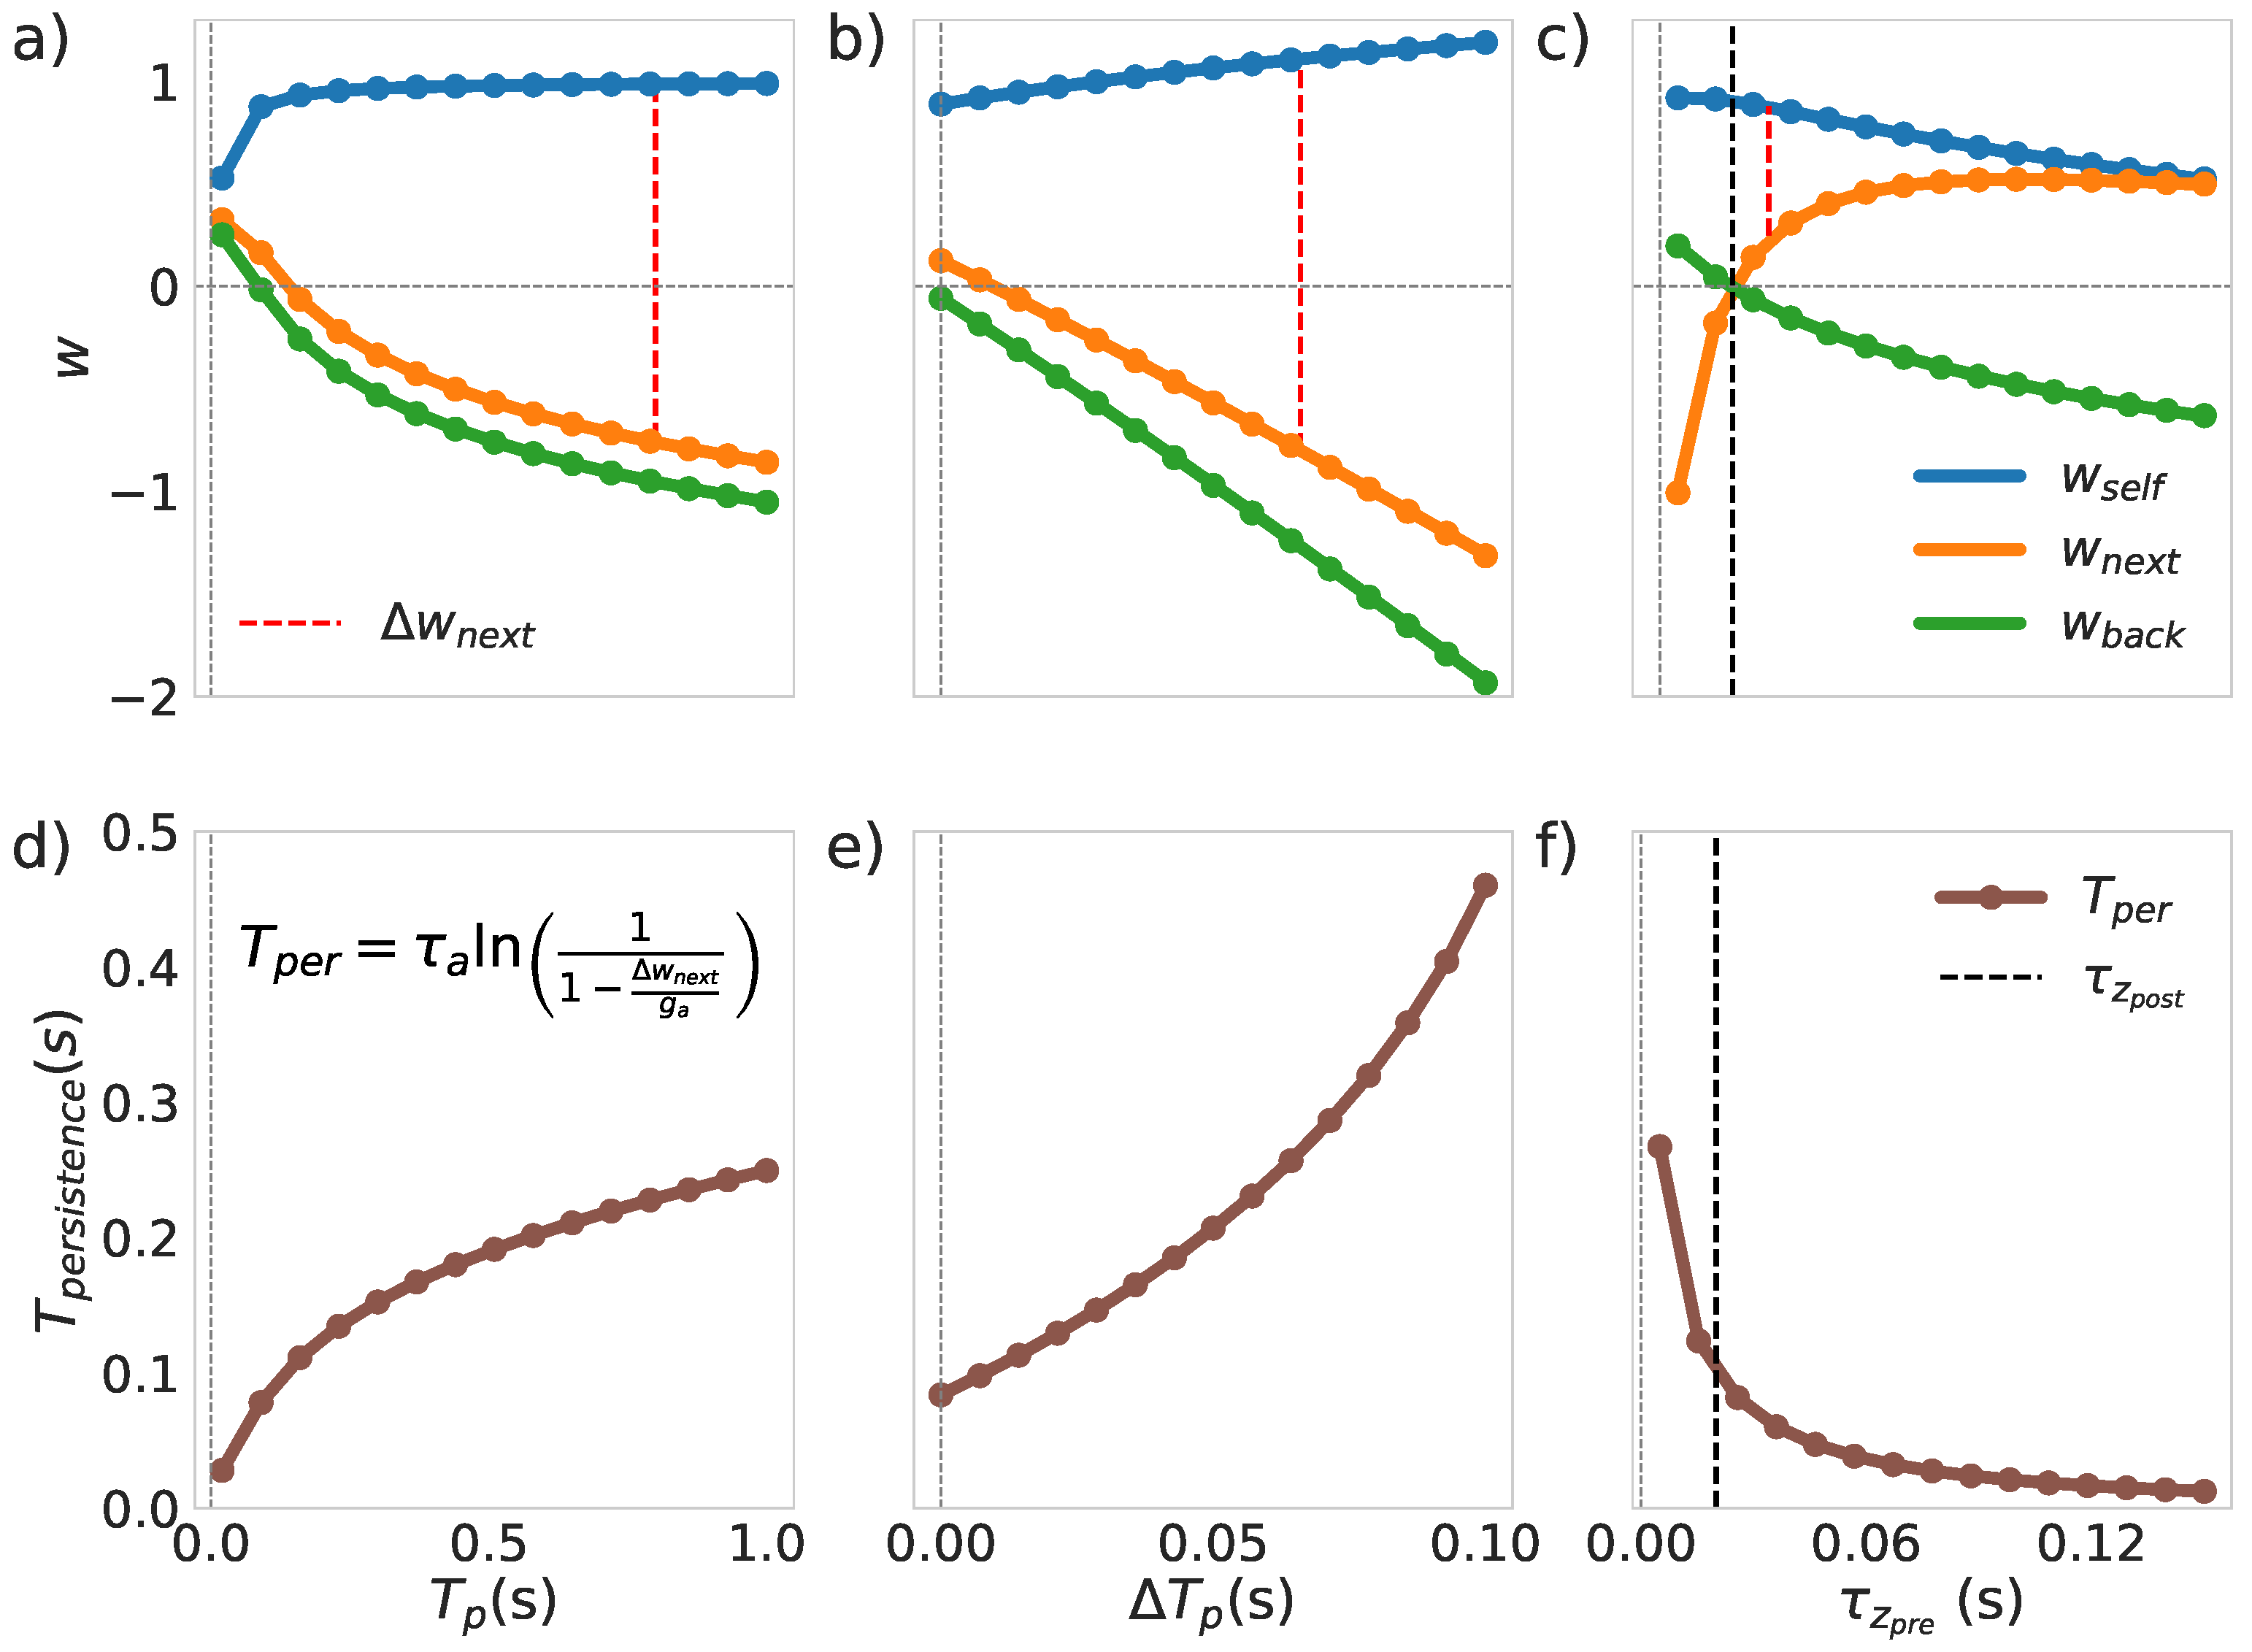
\includegraphics[scale=0.15]{training.pdf}
\caption{A characterization of the connectivity as a function of the protocol}
\label{fig:training}
\end{figure}

\subsection{Noise}

\begin{figure}[H]
\centering
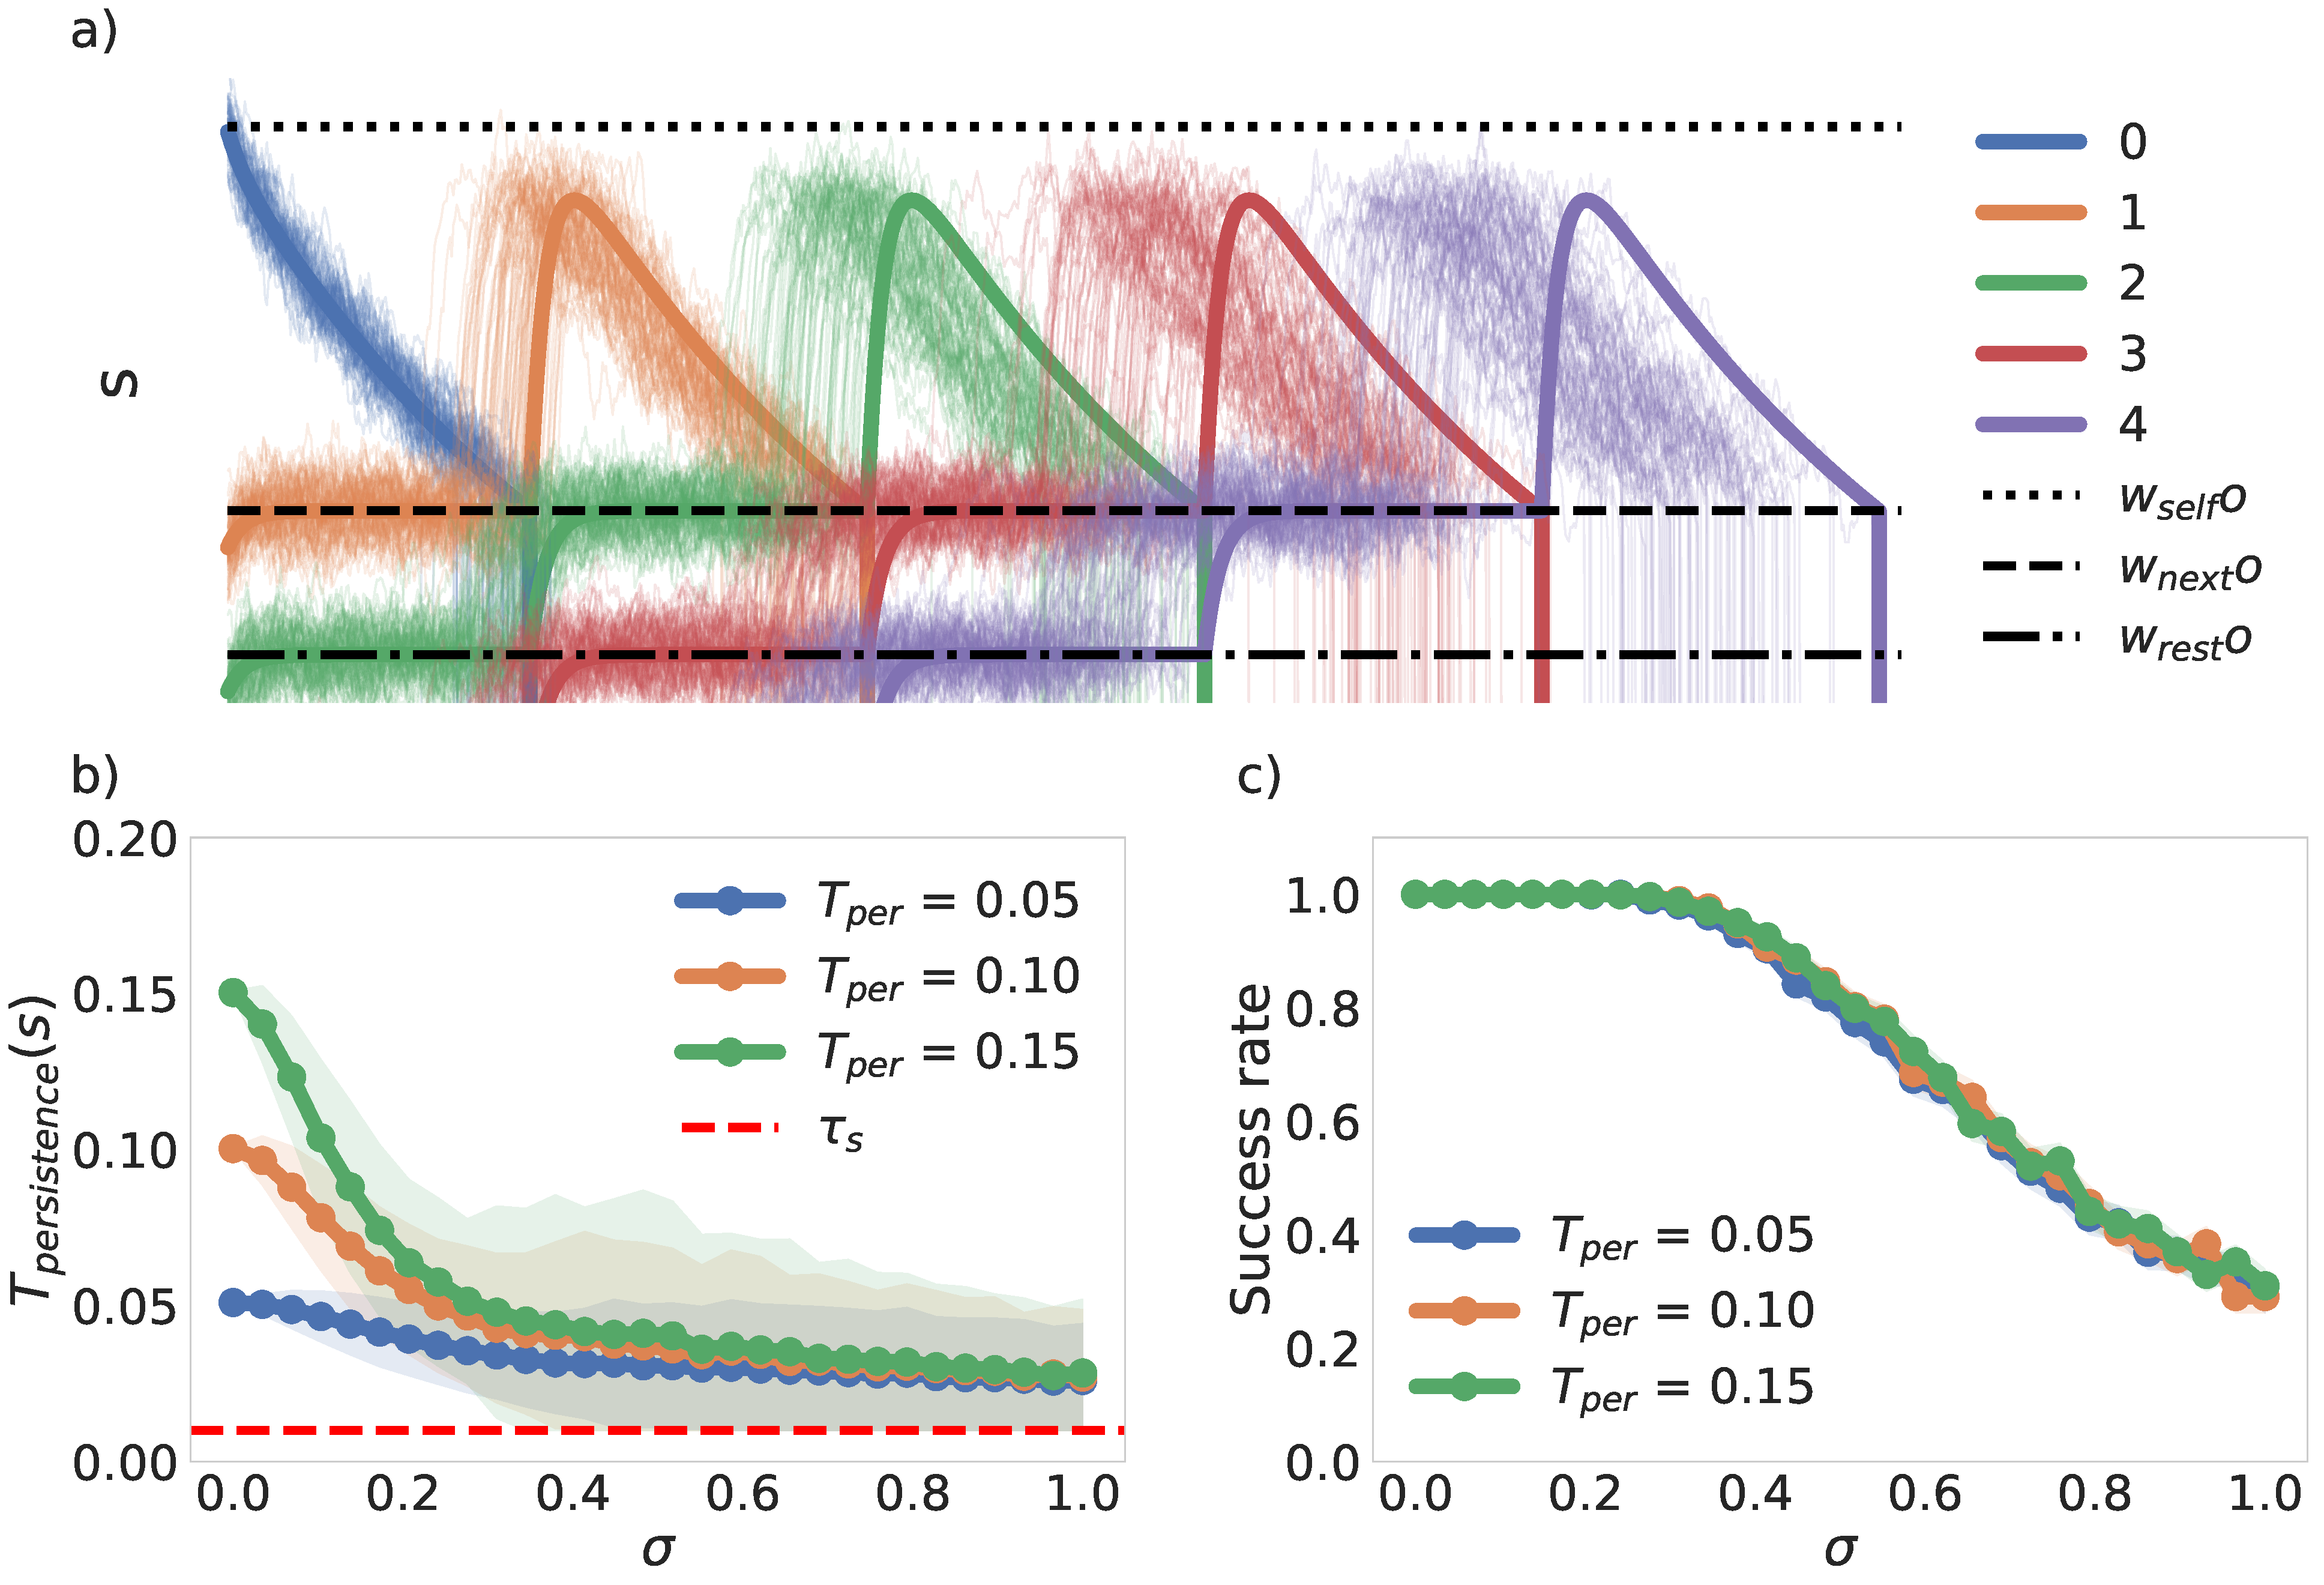
\includegraphics[scale=0.30]{noise_diagram.pdf}
\caption{A schematic of the noise}
\label{fig:noise_scheme}
\end{figure}

\begin{figure}[H]
\centering
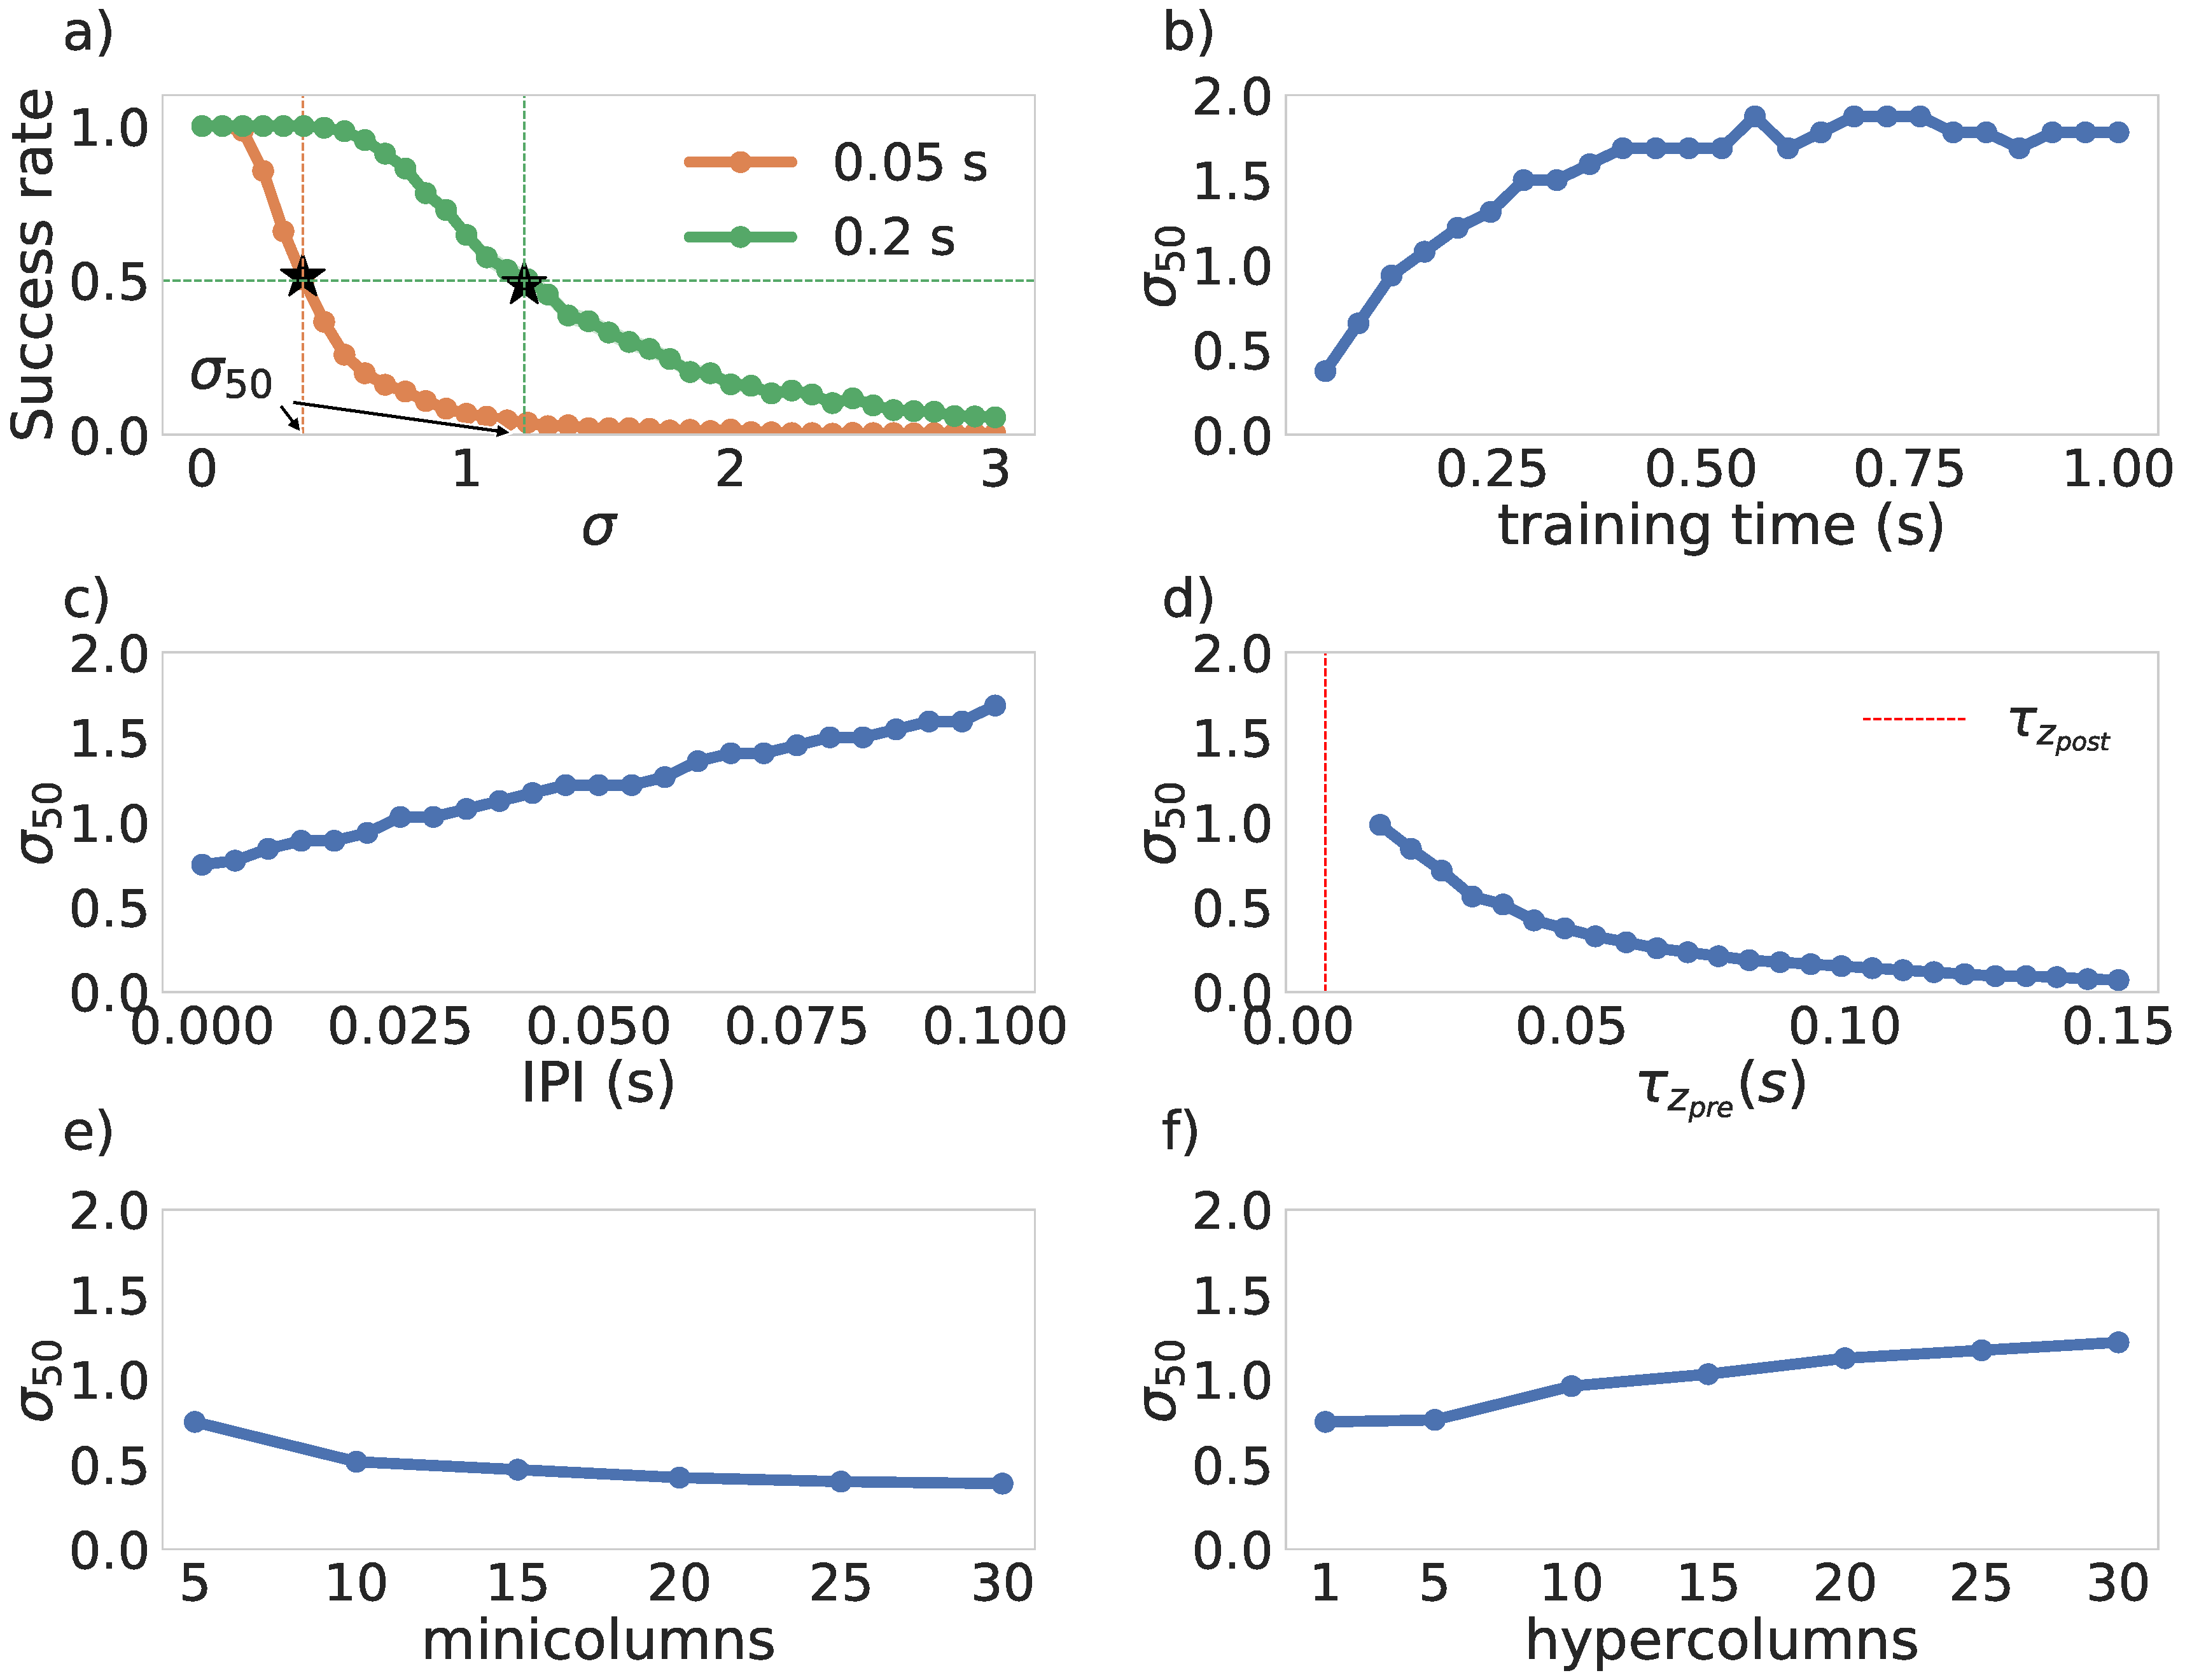
\includegraphics[scale=0.20]{noise_robustness.pdf}
\caption{A characterization of the noise}
\label{fig:robustness}
\end{figure}

\subsection{Representations}
\begin{figure}[H]
\centering
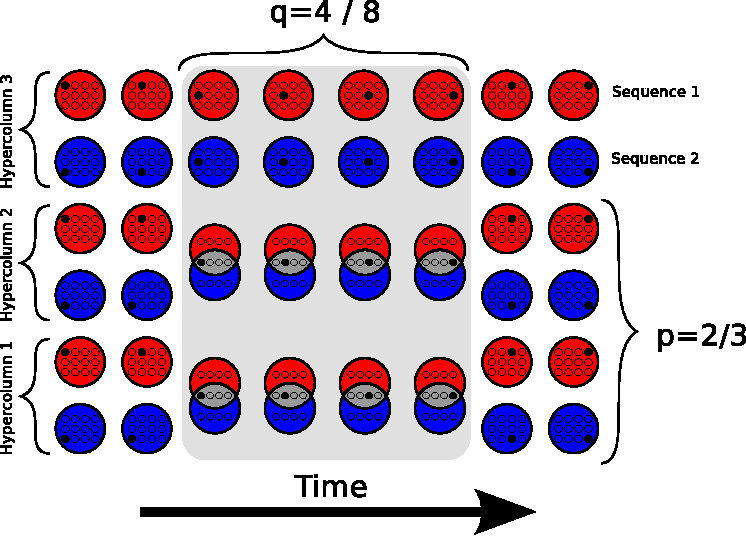
\includegraphics[scale=0.90]{overlap_diagram.pdf}
\caption{Overlap diagram}
\label{fig:representation_scheme}
\end{figure}

\begin{figure}[H]
\centering
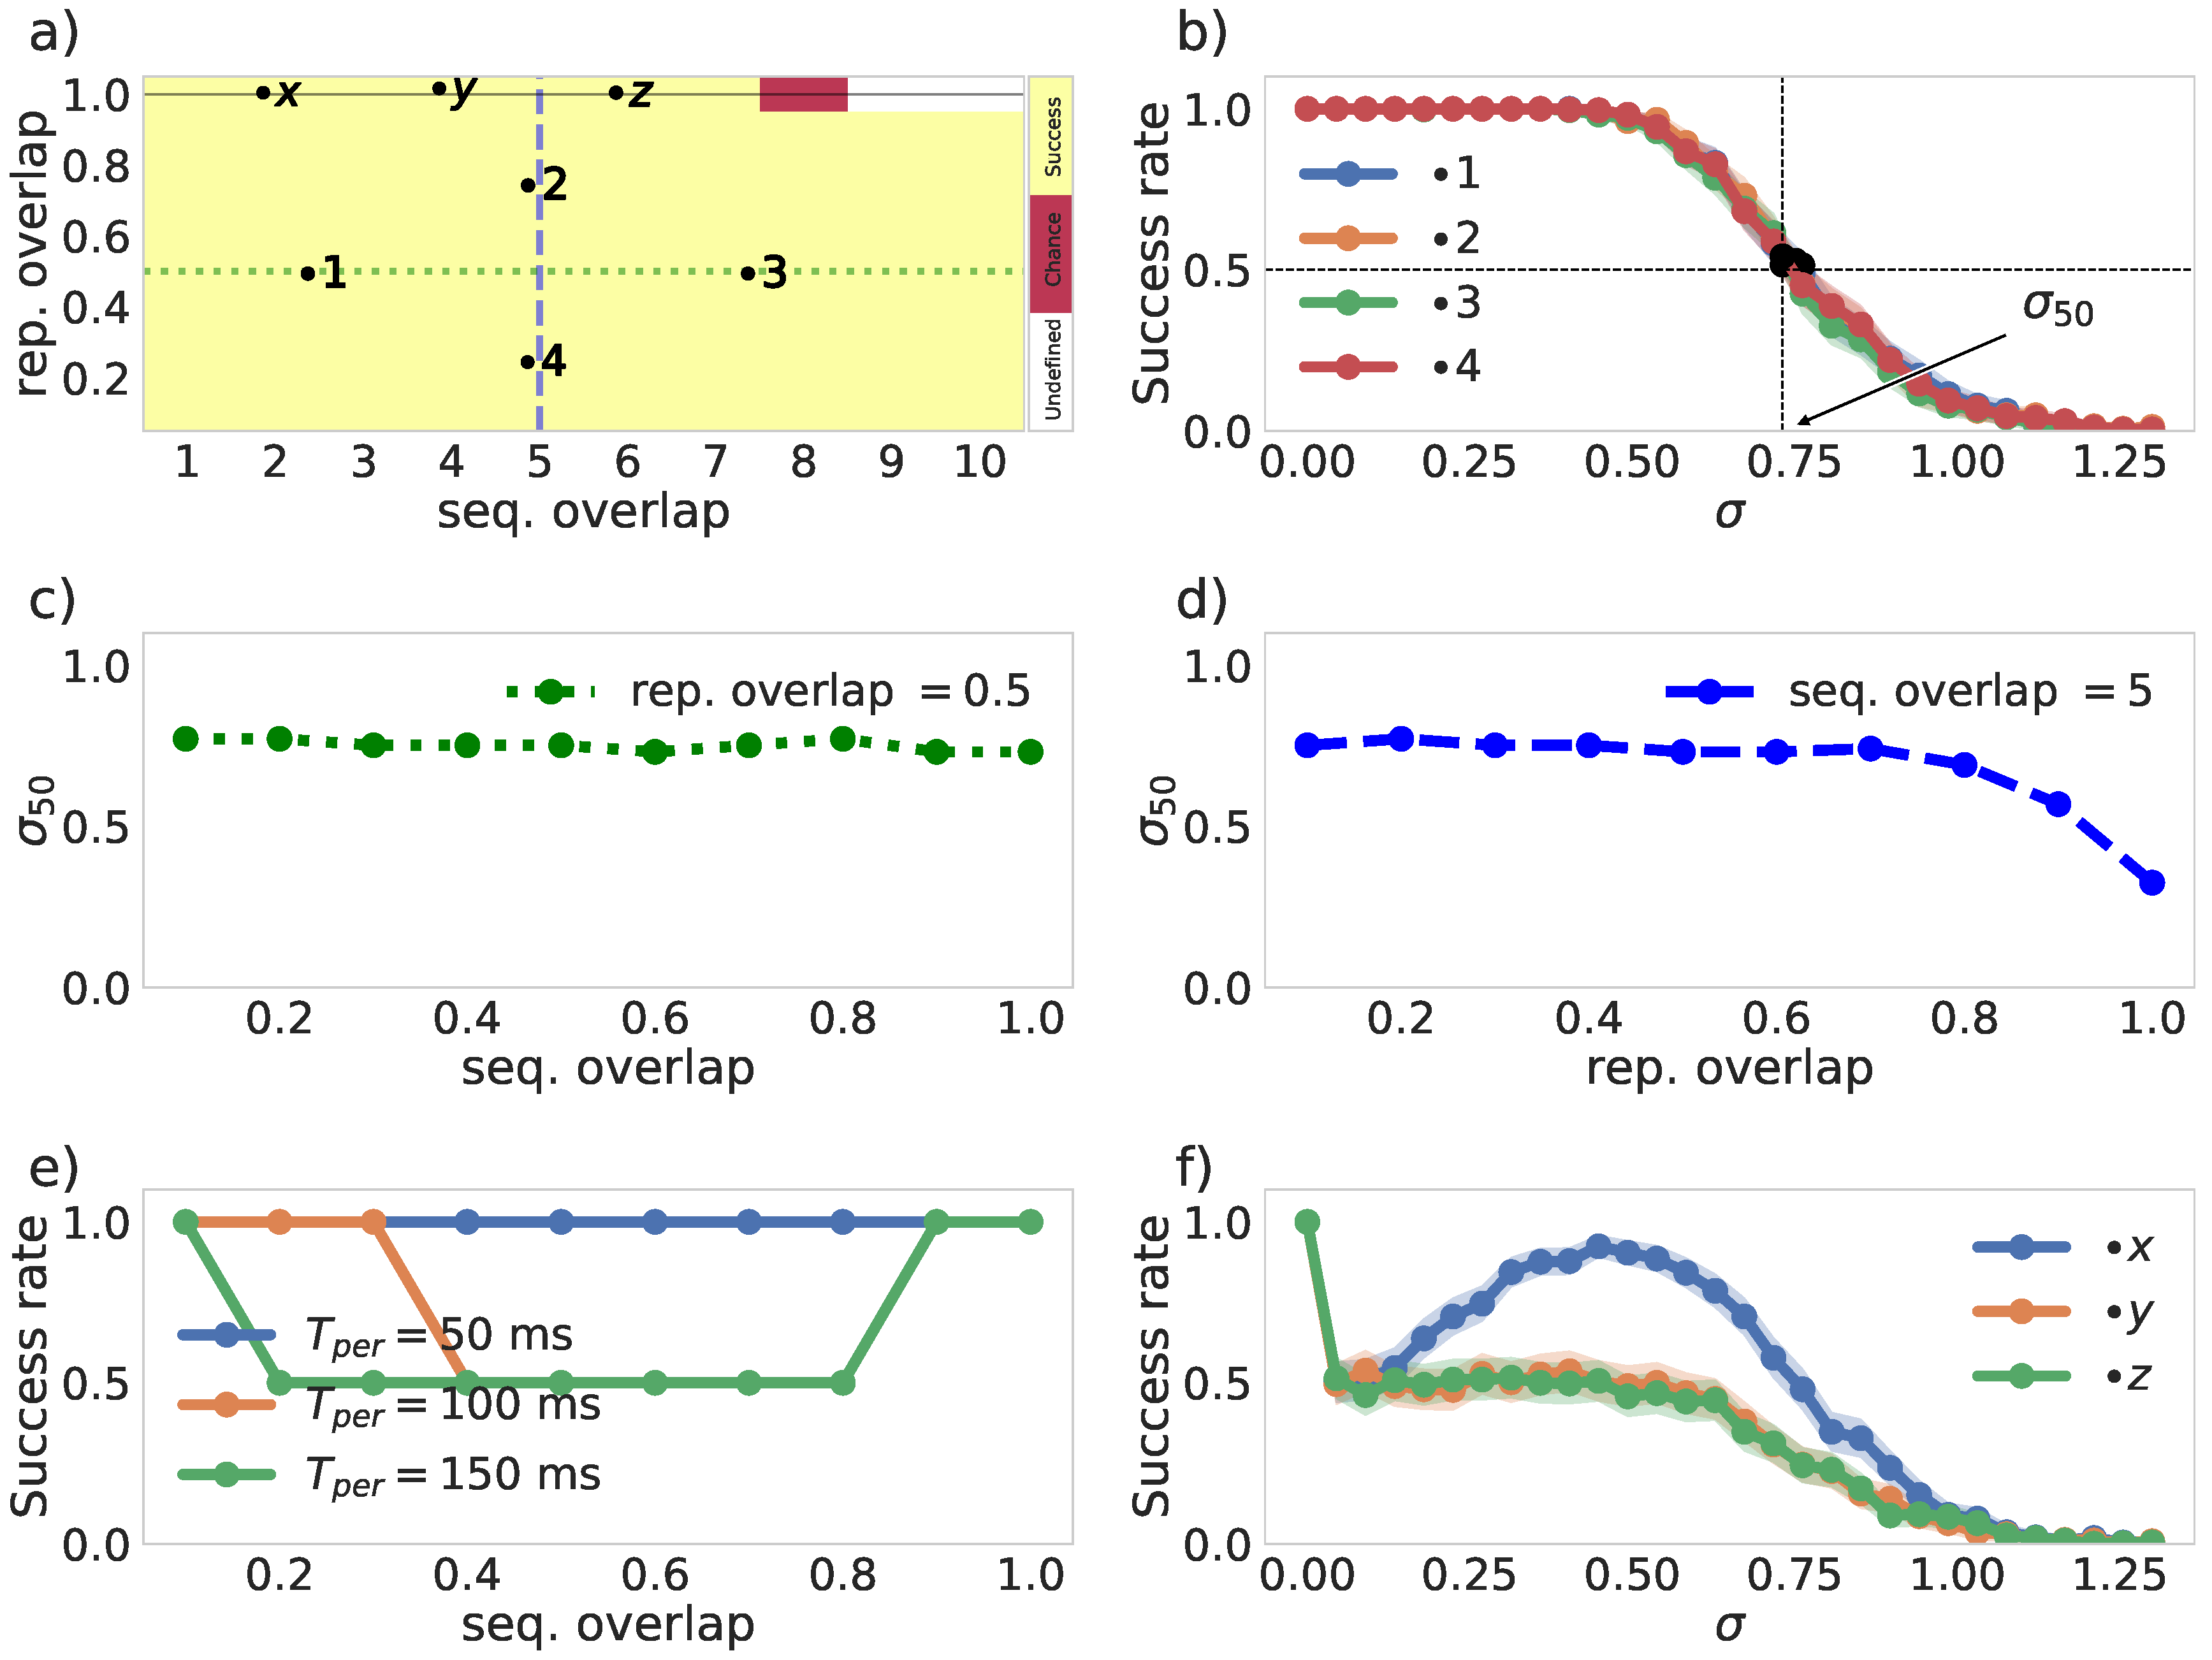
\includegraphics[scale=0.20]{representations.pdf}
\caption{A characterization of the different overlap conditions}
\label{fig:representations}
\end{figure}


\subsection{Non-homogeneous training conditions}

\begin{figure}[H]
\centering
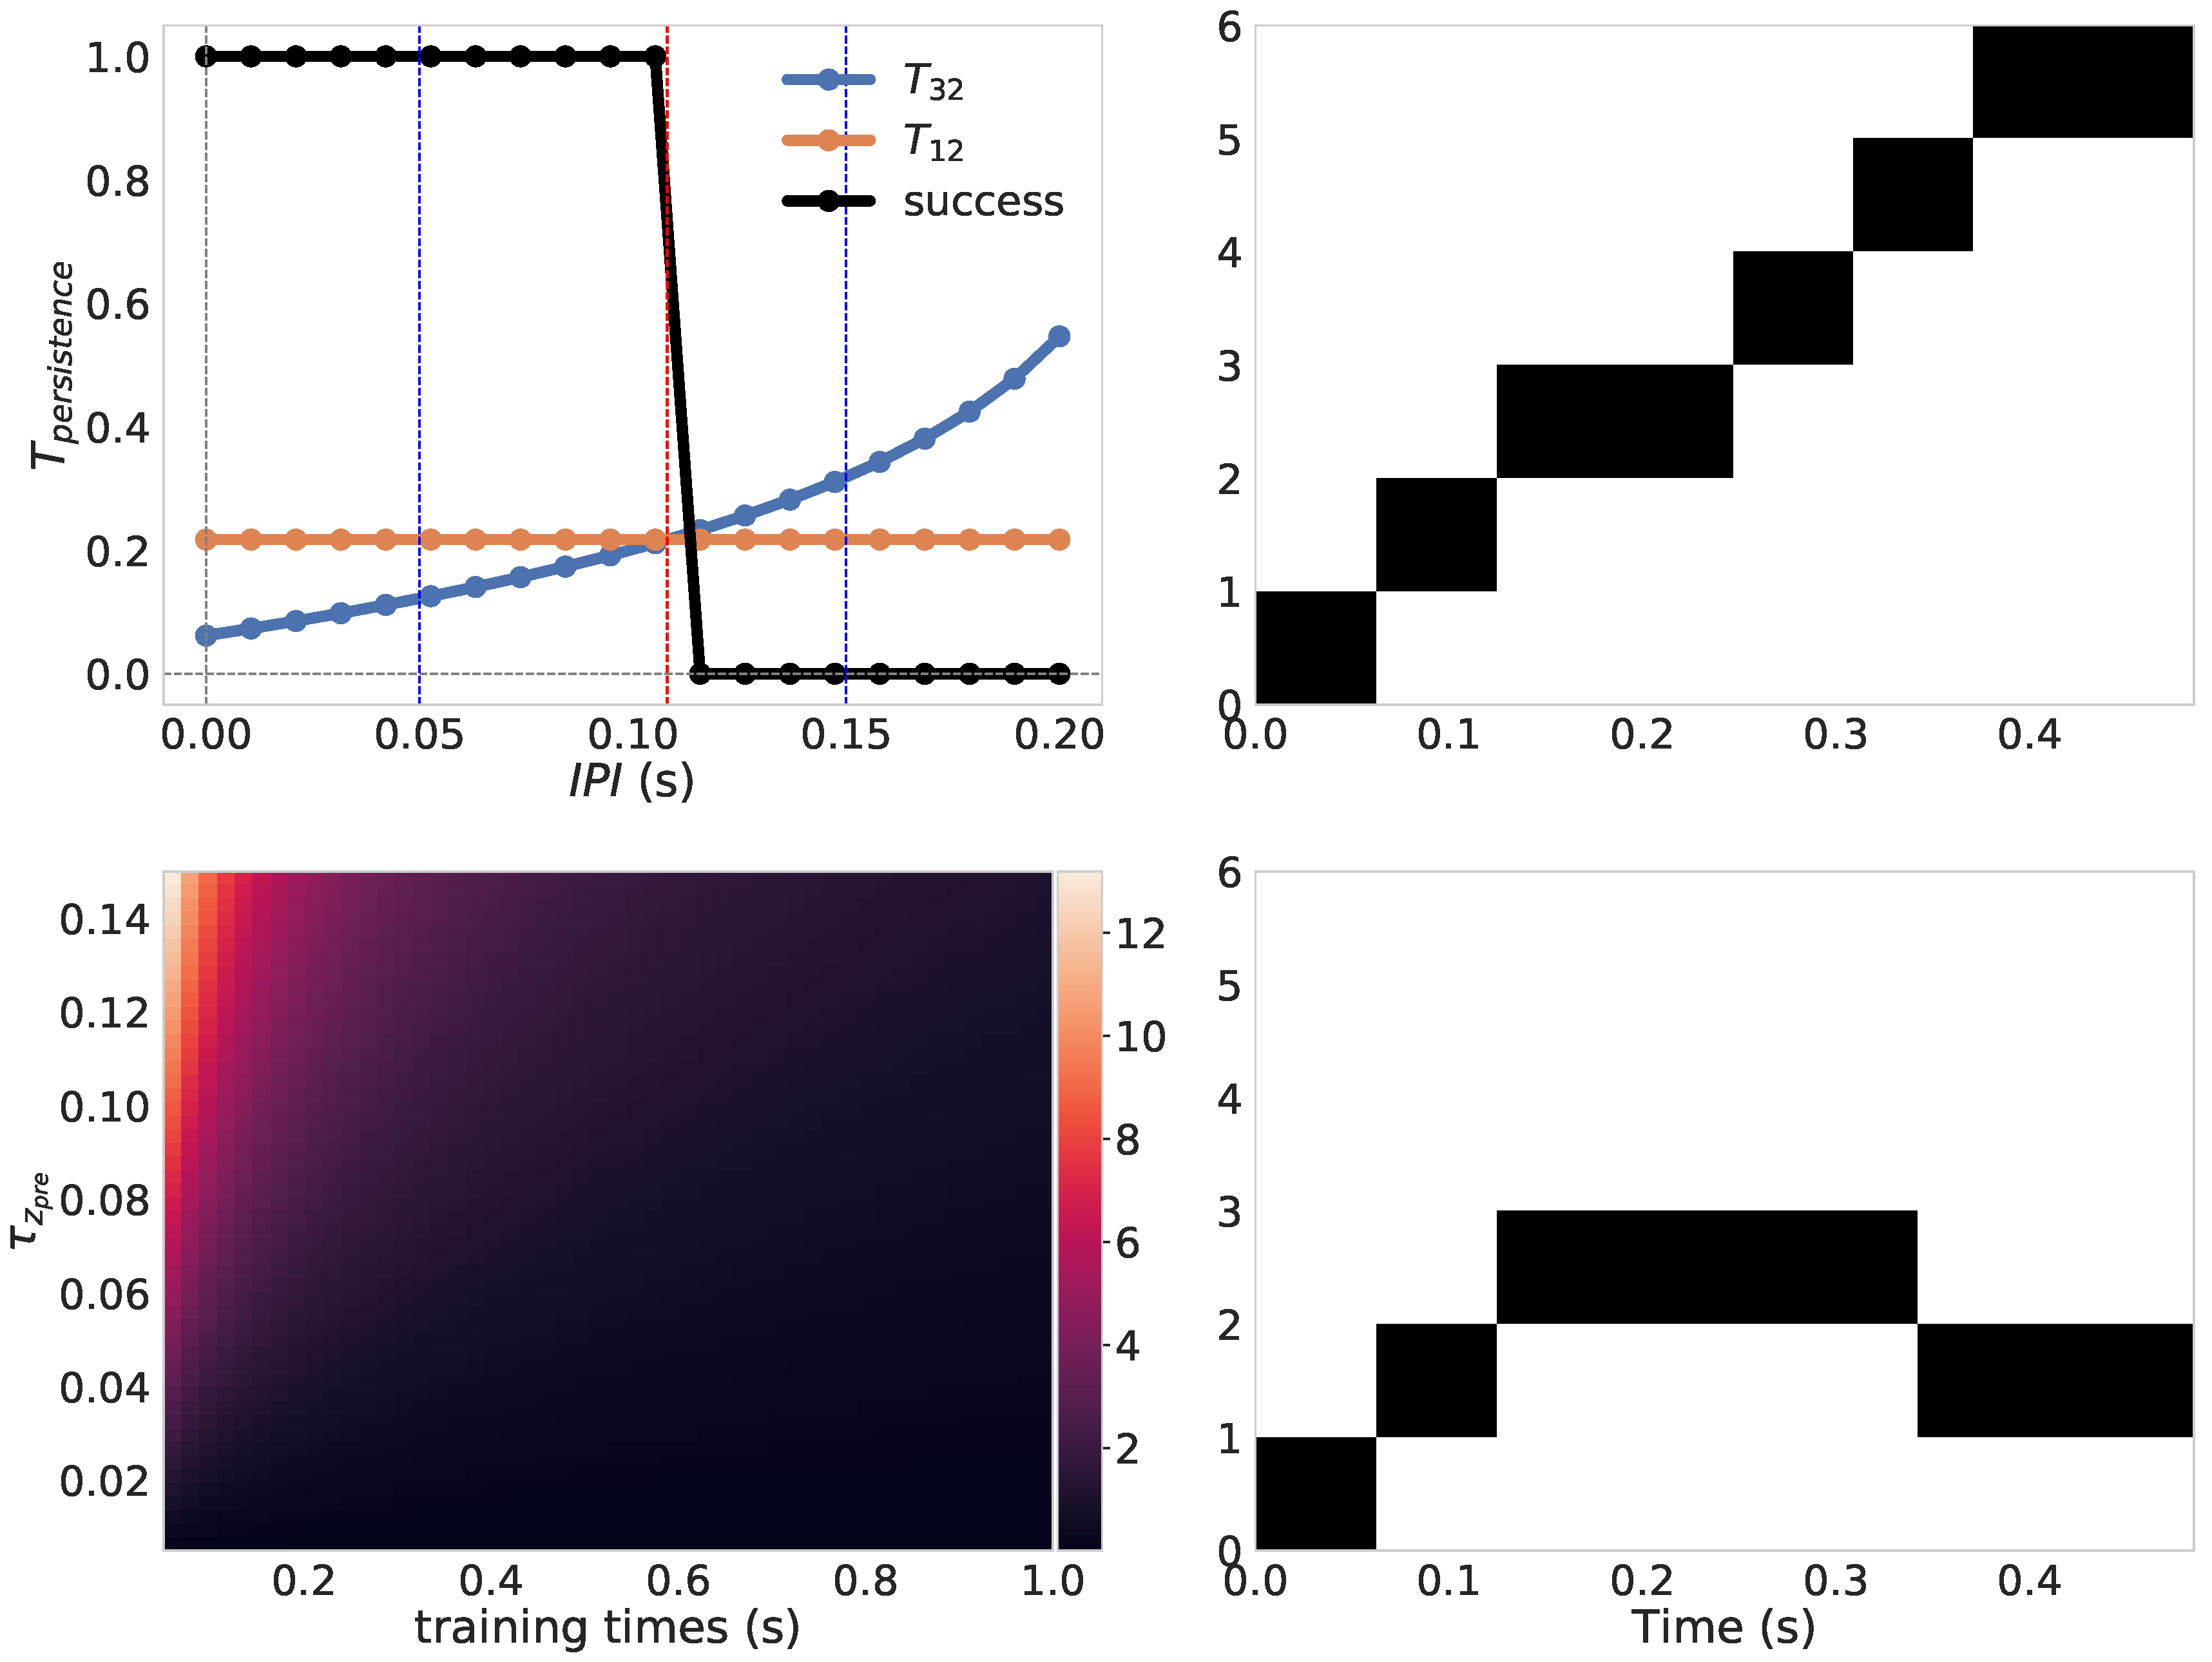
\includegraphics[scale=0.20]{ipi_non_homogenous.pdf}
\caption{A characterization of the different overlap conditions}
\label{fig:non-homo}
\end{figure}


%\bibliographystyle{unsrt}
%\bibliography{references.bib}

\end{document}